\documentclass{beamer}

\mode<presentation>
{
\usetheme{Copenhagen}
%\usetheme{Boadilla}
%\usecolortheme{seahorse}
%\useoutertheme{infolines}
%\useoutertheme[compress]{miniframes}
%\setbeamercovered{transparent}
}

%% \mode<presentation>
%% {
%% \usetheme{progressbar}
%% \setbeamercovered{transparent}
%% }

%\usepackage[english]{babel}
\usepackage[english]{babel}
\usepackage[utf8]{inputenc}
\usepackage[T1]{fontenc}

\usepackage{mathptmx}
\usepackage[scaled=.90]{helvet}
\usepackage[T1]{fontenc}
\usepackage{xspace}
%\usepackage{appendixnumberbeamer}
\usepackage[noend]{algorithmic}
%\usepackage[algo2e,vlined,algochapter,ruled,dotocloa]{algorithm2e}
\usepackage{fancybox}
\usepackage{algorithm}
\usepackage[noend]{algorithmic}
\usepackage{amssymb,amsmath}
% \usepackage{ulem}
\usepackage{makecell}
\usepackage{times}

\title[A few topics in Reinforcement Learning]{From Predictive Maintenance to Machine Learning}
%\title{The Optimal Swapping Problem during Nuclear Refueling Operations}


\author{E. Rachelson}

\institute{
\includegraphics[width=1.5cm]{img/isae.jpg}}

\date{}


% This is only inserted into the PDF information catalog. Can be left
% out.
\subject{From Predictive Maintenance to Machine Learning}

\setbeamerfont{bibliography entry author}{shape=\upshape,series=\bfseries,size=\footnotesize}%
\setbeamerfont{bibliography entry title}{shape=\upshape,size=\scriptsize,series=\mdseries}
\setbeamerfont{bibliography entry journal}{shape=\upshape,size=\scriptsize,series=\mdseries}
\setbeamerfont{bibliography entry note}{shape=\upshape,size=\scriptsize,series=\mdseries}

\setbeamercolor{block}{bg=blue,fg=red}

\beamertemplatenavigationsymbolsempty
\setbeamertemplate{footline}[frame number]

\begin{document}

\begin{frame}[plain]
\titlepage
\end{frame}

\begin{frame}{Schedule}
\begin{enumerate}
\item General introduction\\
Now.
\item Case study\\
This morning.
\item Presentations and discussion\\
Beginning of the afternoon.
\item The Data Scientist point of view\\
The rest of the afternoon.
\end{enumerate}
\end{frame}

\begin{frame}{Course goals}
By the end of the class, you should be able to:
\begin{itemize}
\item explain the workflow of data analysis for Predictive Maintenance problems;
\item know the main bottlenecks and challenges of data-driven approaches to Maintenance;
\item link the Predictive Maintenance problems to their formal Machine Learning counterparts;
\item know the main categories of Machine Learning algorithms and which formal problem they solve;
\item know the name of some key methods in Machine Learning;
\item know the existence of scikit-learn and its API.
\end{itemize}
\end{frame}

\begin{frame}{Course material}
\small\url{https://github.com/erachelson/PredMaintenanceClass}
\end{frame}

\begin{frame}{Case study}
In small groups. Several cases of failure analysis.
\begin{itemize}
\item Turbo-fan engine
\item Air conditioning systems (HVAC)
\item Truck air compressor
\item Pneumatic valve
%\item IOT deployment and railroad use-cases.
%\item Bearings
\end{itemize}
Your task:
\begin{itemize}
\item Prepare a synthesis of your case study (tell the story!).
\item Highlight in particular:
\begin{itemize}
\item nature of data (scalar, booleans, time series, images, text\ldots);
\item properties of data (volume, cleanliness, dimensionnality\ldots);
\item nature of the automated task (visualisation, anomaly detection, RUL prediction\ldots);
\item name of the Machine Learning (and related) methods used;
\item open challenges, bottlenecks.
\end{itemize}
\end{itemize}
\end{frame}

\begin{frame}{Presentations and discussion}
Along the presentations, let's fill the table below, to build a common understanding of:
\begin{itemize}
\item the nature of predictive maintenance data
\item the different tasks to automate
\item the difficulties
\end{itemize}
~\\
~\\
\footnotesize
\begin{tabular}{|c|c|c|c|c|c|}
\hline
\thead{\begin{minipage}{1.3cm}\centering Use case\end{minipage}} & \thead{\begin{minipage}{1.3cm}\centering Type of data\end{minipage}} & \begin{minipage}{1.3cm}\centering Properties of data\end{minipage} & \begin{minipage}{1.3cm}\centering Task to automate\end{minipage} & \begin{minipage}{1.3cm}\centering Difficulties\end{minipage} & \begin{minipage}{1.3cm}\centering Comments\end{minipage}\\
\hline
 & & & & & \\
\hline
 & & & & & \\
\hline
 & & & & & \\
\hline
 & & & & & \\
\hline
\end{tabular}
\end{frame}

\begin{frame}{The Data Scientist perspective}
\centering 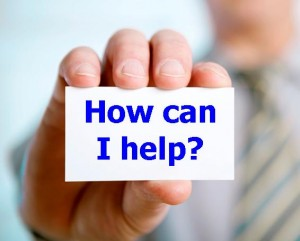
\includegraphics[width=6cm]{img/How-can-i-help.jpg}
\end{frame}

\begin{frame}{Identified needs}
We would like to build automated tools for the following tasks:
\begin{itemize}
\item Visualize system state
\item Identify anomalies
\item Predict Remaining Useful Life (RUL) / Time To Failure (TTF)
\item Predict failure occurrence or probability at a given horizon
\end{itemize}
All this, in order to base our maintenance strategy on the (inferred) system state, rather than a general statistical trend.\\
~\\
Traditionaly, all this is based on user expertise.\\
Let's take a data-driven approach.
\end{frame}

\begin{frame}{Data analysis workflow for Predictive Maintenance}
\begin{enumerate}
\item<1-> Collect
\item<2-> Analyze
\item<3-> Predict
\item<4-> React
\end{enumerate}
\begin{overlayarea}{10cm}{4cm}
\begin{block}{}
\only<1>{
\begin{itemize}
\item Sensors deployment
\item Historical data collection
\item Integrated storage and retrieval issues
\end{itemize}
$\rightarrow$ Extract-Transform-Load (ETL) process
}
\only<2>{
\begin{itemize}
\item data cleaning
\item feature selection / engineering
\item algorithm selection
\item parameters tuning
\end{itemize}
}
\only<3>{
\begin{itemize}
\item Make predictions on new test cases
\item Deploy solution in your operational process
\item Make things usable
\end{itemize}
}
\only<4>{
\begin{itemize}
\item Improve your maintenance decisions
\end{itemize}
}
\only<5>{
Need to automate as many steps as possible in this workflow\\
\hspace{2cm}$\rightarrow$ data-driven approaches\\
\hspace{2cm}$\rightarrow$ Machine Learning for step 2 (and 3)
}
\end{block}
\end{overlayarea}
\end{frame}

\begin{frame}{A word on data quality}
\begin{itemize}
\item amount of data: data is often abundant but crucial data is often scarce
\item noise, errors, missing data, outdated data: reliability
\item high-dimensional data
\item class imbalance
\item heterogeneous data (scalars, booleans, time series, images, text, \ldots)
\end{itemize}
All these will influence your algorithmic design or choices.\\
~\\
So let's talk about algorithms to see how we can solve the PM problems listed earlier.
\end{frame}

\begin{frame}{Machine Learning}
\centering
Machines that learn?\\
Let's try to give a general definition.\\
~\\
\visible<2>{Machine learning is a field of computer science that gives computer systems the ability to ``learn'' (i.e. progressively improve performance on a specific task) with data, without being explicitly programmed.}
\end{frame}

\begin{frame}{ML examples}
\begin{overlayarea}{\textwidth}{5cm}
\begin{itemize}
\item<1-> Given 20 years of clinical data, will this patient have a second heart attack in the next 5 years?
\item<2-> What price for this stock, 6 months from now?
\item<3-> Is this handwritten number a 7?
\item<4-> Is this e-mail a spam?
\item<5-> Can I cluster together customers? press articles? genes?
\item<6-> What is the best strategy when playing Counter Strike? or poker?
\end{itemize}
\end{overlayarea}
\begin{overlayarea}{\textwidth}{2.5cm}
\begin{center}
\only<1>{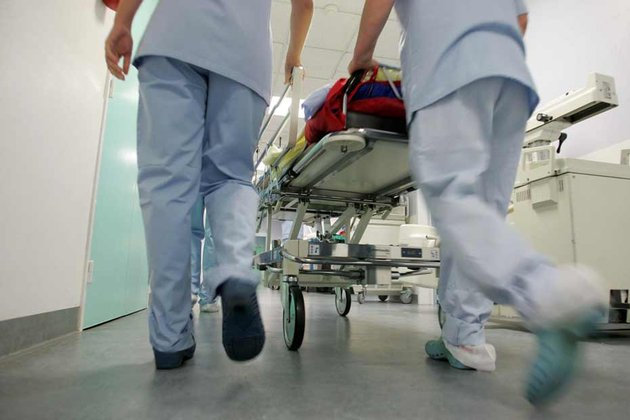
\includegraphics[height=2.5cm]{img/hopital.jpg}}
\only<2>{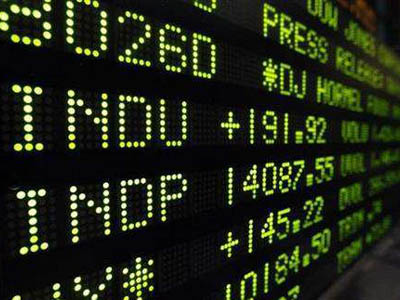
\includegraphics[height=2.5cm]{img/finance.jpg}}
\only<3>{
\includegraphics[height=2.5cm]{img/seven.jpg}}
\only<4>{\begin{tabular}{rl}
\begin{minipage}{0.9cm}

\includegraphics[height=1cm]{img/message.jpg}
\end{minipage} & \textbf{Enlarge your thesis!}
\end{tabular}}
\only<5>{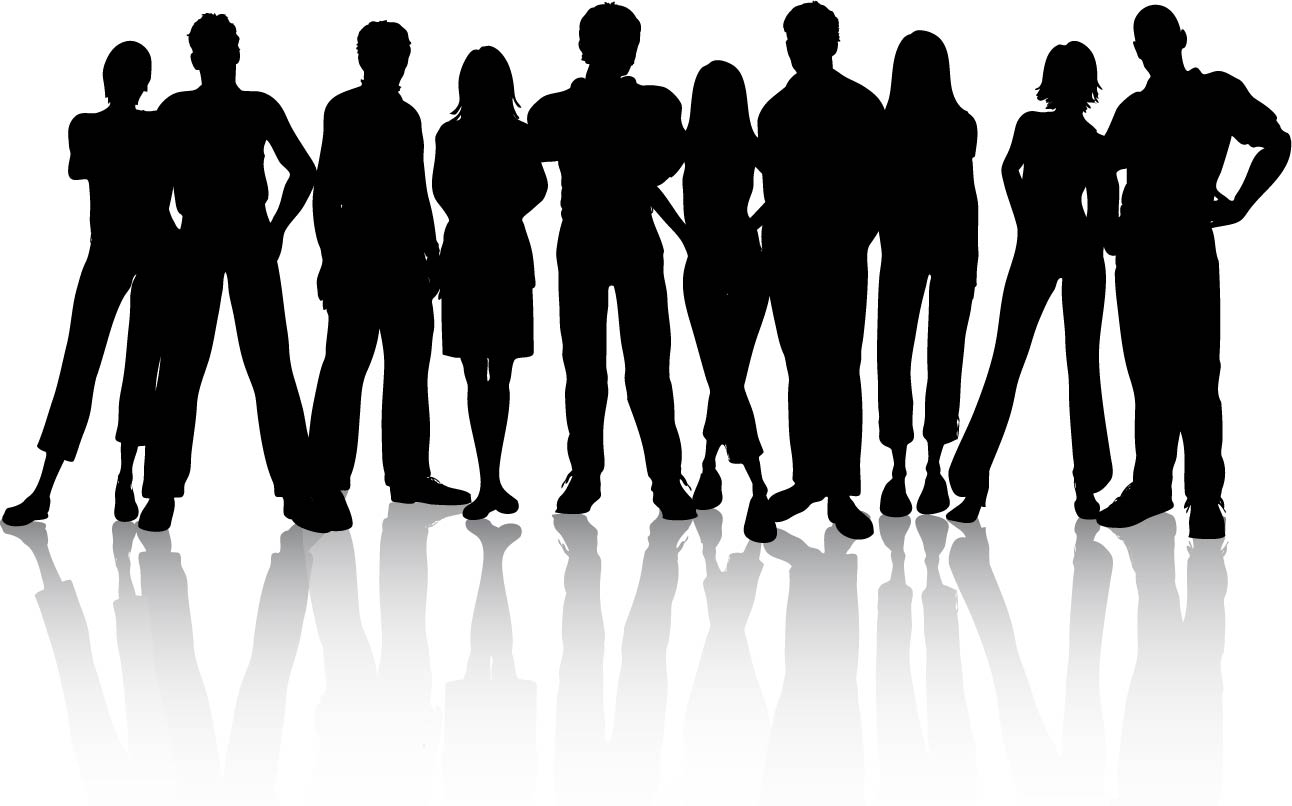
\includegraphics[height=2.5cm]{img/people.jpg}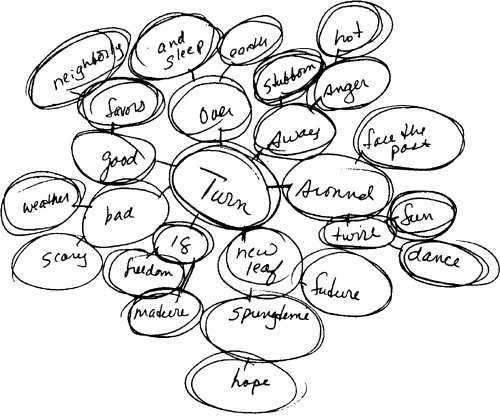
\includegraphics[height=2.5cm]{img/words.jpg}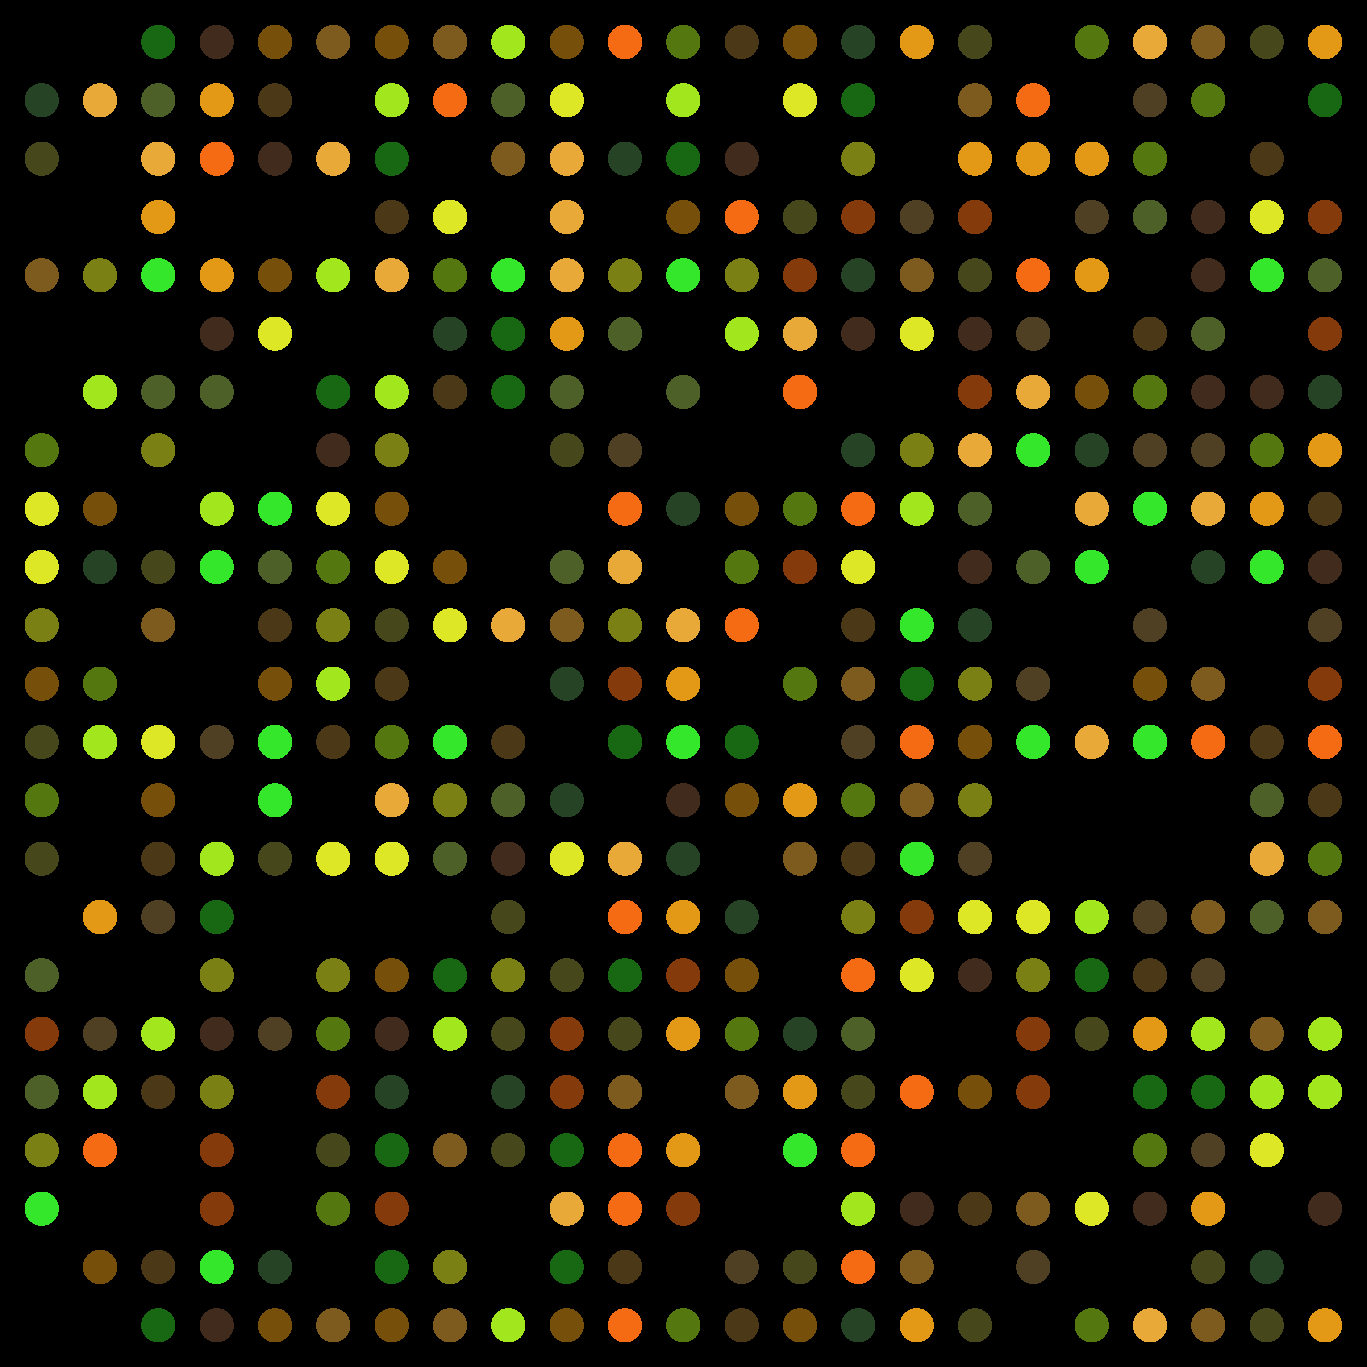
\includegraphics[height=2.5cm]{img/DNA_microarray.pdf}}
\only<6>{
\includegraphics[height=2.5cm]{img/counterstrike.jpg}~~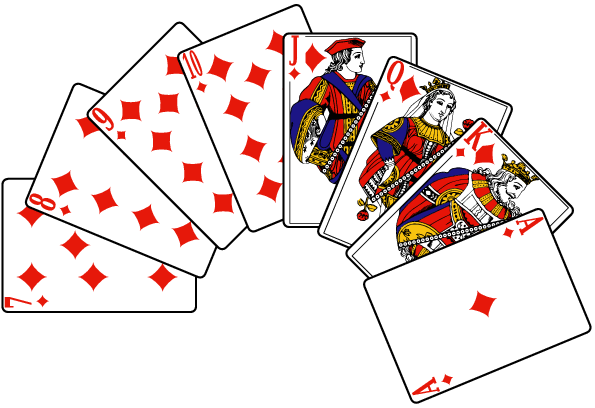
\includegraphics[height=2.5cm]{img/cartes.png}}
\end{center}
\end{overlayarea}
\end{frame}

\begin{frame}{ML tasks}
What does ML do? 3 main tasks.\\
~\\
\begin{tabular}{|c|c|c|c|}
\hline
\makecell[{{p{0.07\textwidth}}}]{\textbf{Task}} &
\makecell[{{p{0.27\textwidth}}}]{\centering Supervized\\ Learning} & \makecell[{{p{0.27\textwidth}}}]{\centering Unsupervized Learning} & \makecell[{{p{0.27\textwidth}}}]{\centering Reinforcement Learning}\\
\hline
\makecell[{{p{0.07\textwidth}}}]{\textbf{Goal}} &
\makecell[{{p{0.27\textwidth}}}]{\centering Learn a function, $f(x)=y$} & \makecell[{{p{0.27\textwidth}}}]{\centering Find groups and correlations, $x\in C$} & \makecell[{{p{0.27\textwidth}}}]{\centering Optimal control, $f(x)=u \ / \ \max\sum r$}\\
\hline
\makecell[{{p{0.07\textwidth}}}]{\textbf{Data}} &
\makecell[{{p{0.27\textwidth}}}]{\centering $\{(x,y)\}$} & \makecell[{{p{0.27\textwidth}}}]{\centering $\{x\}$} & \makecell[{{p{0.27\textwidth}}}]{\centering $\{(x,u,r,x')\}$}\\
\hline
\makecell[{{p{0.07\textwidth}}}]{\textbf{Sub-task}} &
\makecell[{{p{0.27\textwidth}}}]{\centering Classification, Regression} & \makecell[{{p{0.27\textwidth}}}]{\centering Clustering, Density estimation, Dimensionnality reduction} & \makecell[{{p{0.27\textwidth}}}]{\centering Value estimation, Policy optimization}\\
\hline
\makecell[{{p{0.07\textwidth}}}]{\textbf{Algo ex.}} &
\makecell[{{p{0.27\textwidth}}}]{\centering Neural Networks, SVM, Random Forests} & \makecell[{{p{0.27\textwidth}}}]{\centering k-means, PCA, HCA} & \makecell[{{p{0.27\textwidth}}}]{\centering Q-learning}\\
\hline
\end{tabular}
\end{frame}

\begin{frame}{Misconceptions and clarifications}
\begin{itemize}
\item[AI] ML is only a small (currently fashionable) part of Artificial Intelligence.
\item[BD] Big Data refers to working with datasets that have large Volume, Variety, Velocity (, Veracity, and Value).
\item[DL] Deep Learning is Machine Learning with Deep Neural Networks.
\item[threat] ML / Data Science / Big Data are as much of a threat (to jobs, the society, the economy\ldots) as the combustion engine was in the XIXth century.
\end{itemize}
\end{frame}

\begin{frame}{ML software}
Software:
\begin{itemize}
\item Many free libraries: scikit-learn, tensorflow, caffe\ldots check \url{www.mloss.org} if you're curious.
\item Free environments: Weka, RStudio\ldots
\item Commercial embedded solutions (more or less specialized): Matlab, IBM, emaint, Microsoft\ldots
\end{itemize}
\end{frame}

%% \begin{frame}{Evaluation}
%% Evaluating ML methods?
%% \begin{itemize}
%% \item Regression: RMSE, margin \ldots
%% \item Classification: Misclass rate, TP, FP, cross entropy, ROC\ldots
%% \item Clustering: similarity scores
%% \end{itemize}
%% \end{frame}

\begin{frame}{The process of (Un)Supervized Learning}
\begin{center}
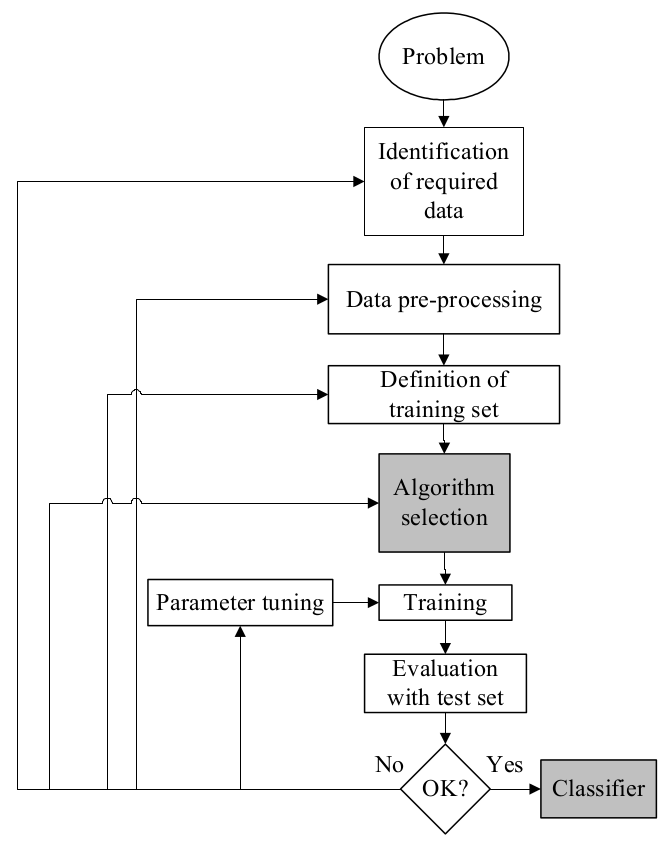
\includegraphics[height=7cm]{img/process.png}
\end{center}
\vspace{-0.5cm}
{\footnotesize From \textbf{Supervized Machine Learning: A Review of Classification Techniques}, S. B. Kotsiantis, \textit{Informatica}, 31:249--268, 2007.}
\end{frame}

\begin{frame}{Relating PM and ML}
\visible<1->{
\begin{itemize}
\item Visualizing system state\\
\hspace{1cm} $\rightarrow$ Dimensionnality reduction (Unsupervized learning)
\item Detecting anomalies\\
\hspace{1cm} $\rightarrow$ Density estimation (Unsupervized learning)
\item Predicting RUL or TTF\\
\hspace{1cm} $\rightarrow$ Regression (Supervized learning)
\item Predicting failure in $N$ cycles\\
\hspace{1cm} $\rightarrow$ Classification (Supervized learning)
\end{itemize}
}
\visible<2->{
~\\
Thinking like a Maintenance Engineer:\\
How can I monitor my system to manage my maintenance operations?\\
Thinking like a Data Scientist:\\
Is this a supervized or unsupervized problem? What available data?\\
~\\
Now you can start discussing with data scientists to design together the most appropriate method for your data and your problem.
}
\end{frame}

\begin{frame}{A word on scikit-learn}
Scikit-learn = Machine Learning in Python
\begin{itemize}
\item Simple and efficient tools for data mining and data analysis
\item Accessible to everybody, and reusable in various contexts
\item Built on NumPy, SciPy, and matplotlib
\item Open source, commercially usable - BSD license
\item Well documented, with lots of examples
\end{itemize}
\url{http://scikit-learn.org}\\
~\\
Let's take a look at the \href{http://scikit-learn.org/stable/user_guide.html}{documentation's table of contents} to grasp a few more keywords.
\end{frame}

\begin{frame}{Course goals}
By the end of the class, you should be able to:
\begin{itemize}
\item explain the workflow of data analysis for Predictive Maintenance problems;
\item know the main bottlenecks and challenges of data-driven approaches to Maintenance;
\item link the Predictive Maintenance problems to their formal Machine Learning counterparts;
\item know the main categories of Machine Learning algorithms and which formal problem they solve;
\item know the name of some key methods in Machine Learning;
\item know the existence of scikit-learn and its API.
\end{itemize}
\end{frame}

\begin{frame}{Let's finish with a focus on a practical use-case}
The ``digits'' dataset.
\vspace{-0.3cm}
\begin{center}
\begin{tabular}{ccc}
\begin{minipage}{3cm}
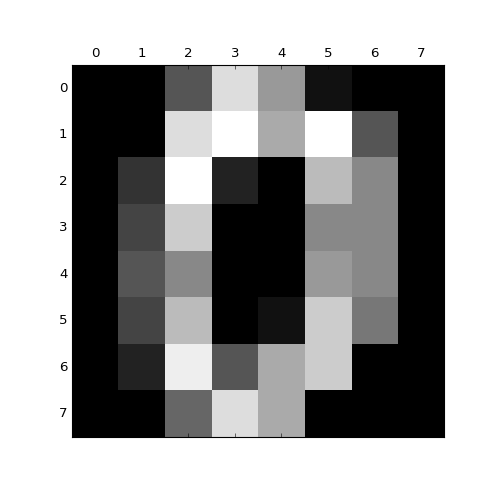
\includegraphics[width=3cm]{img/digits0.png}
\end{minipage} &
\begin{minipage}{3cm}
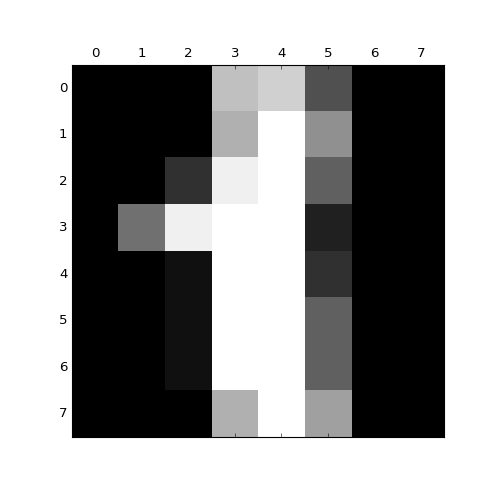
\includegraphics[width=3cm]{img/digits1.png}
\end{minipage} &
\begin{minipage}{3cm}
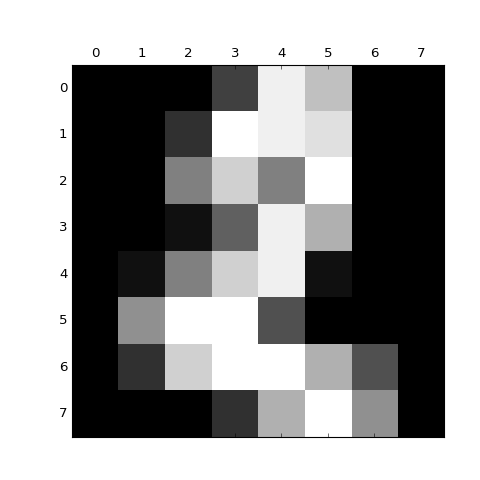
\includegraphics[width=3cm]{img/digits2.png}
\end{minipage} \\
\begin{minipage}{3cm}
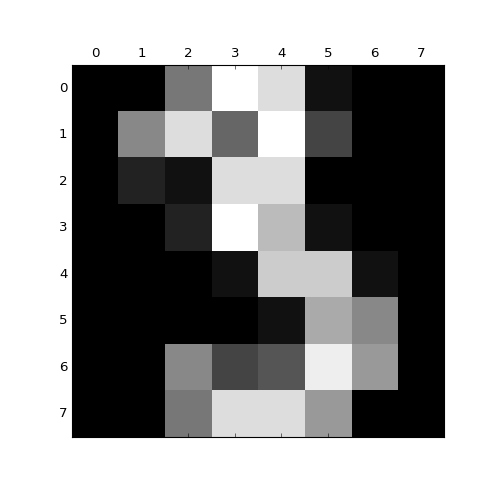
\includegraphics[width=3cm]{img/digits3.png}
\end{minipage} &
\begin{minipage}{3cm}
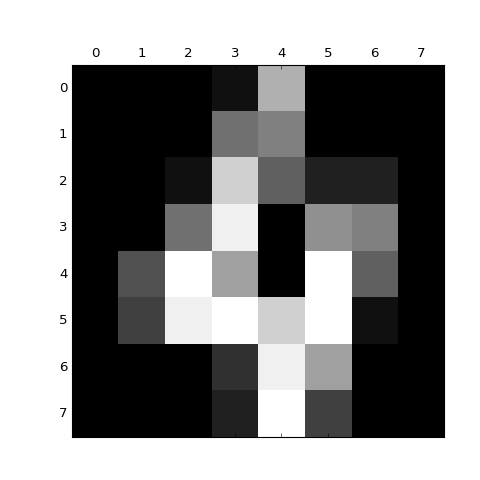
\includegraphics[width=3cm]{img/digits4.png}
\end{minipage} &
\begin{minipage}{3cm}
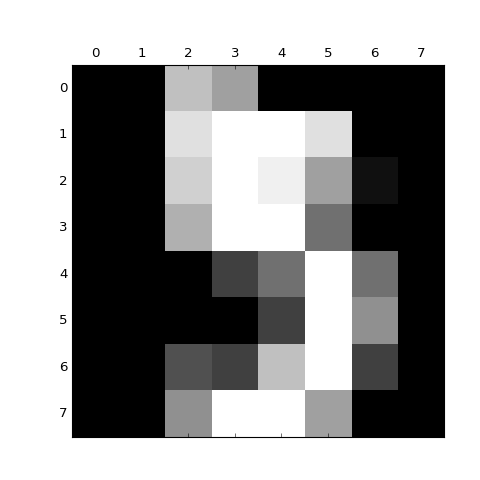
\includegraphics[width=3cm]{img/digits5.png}
\end{minipage}
\end{tabular}
\end{center}
Voluntarily not directly a maintenance case, because:
\begin{itemize}
\item the data you're likely to encounter might often surprise you;
\item it's easy to visualize things with this example.
\end{itemize}
\end{frame}

\end{document}
